\chapter[Scale-up]%
{Scale-up}
\label{Scale-up}

\section{Analysis of a non reactive flow in a basic case}

\begin{figure}[!h]
  \centering
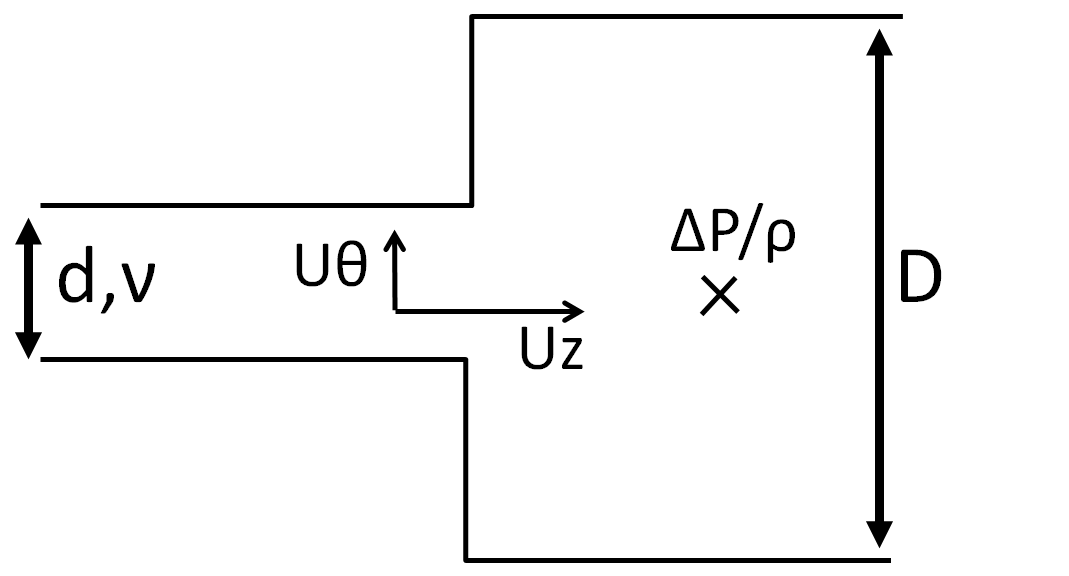
\includegraphics[width=0.6\textwidth]{fig/Schema_Vashy1.png}
  \caption{Basic case}
 \label{Vaschy1}
\end{figure}
Given a burner of internal diameter $d$, with a bulk velocity $u_{z}$,a tangential velocity $u_{\theta}$ ,  followed by a combustion chamber of internal diameter $D$, and a fluid with a cinematic viscosity $\nu$, we what to describe the behavior of the non-reactive flow inside the furnace. For instance, we can study the quantity $\frac{\Delta P}{\rho}$ at a given point inside the combustion chamber, we can otherwise choose $u_{r}$or any physical values, the adimensional numbers will be the same.

We need hypothesis for the velocities : let's assume a top-hat axial velocity, and a solid block body rotation, giving the shape :$u_{\theta}=\Omega r$. Let us use the Vaschy-Buckingham Theorem : we assume that the flow (through the quantity $\frac{\Delta P}{\rho}$ ) only depends on the previous data. 

Since we have 5 independent inputs, with 2 units, there are $5-2=3$ adimensional numbers which fully describes the non-reactive flow. We can guess them, or find it back with linear analysis :
\begin{itemize}
\item $Re$ 
\item $S=\frac{\Omega D}{u_{z}}$
\item $C=\frac{d}{D}$
\end{itemize}
The flow is only a function of $S$, $Re$ and $C$ . The adimensional numbers can vary linearly to these previous quantities, but the combinations of the physical inputs is unique.

\section{In the case of non uniform fields depending on cylindrical coordinates}

\begin{figure}[!h]
  \centering
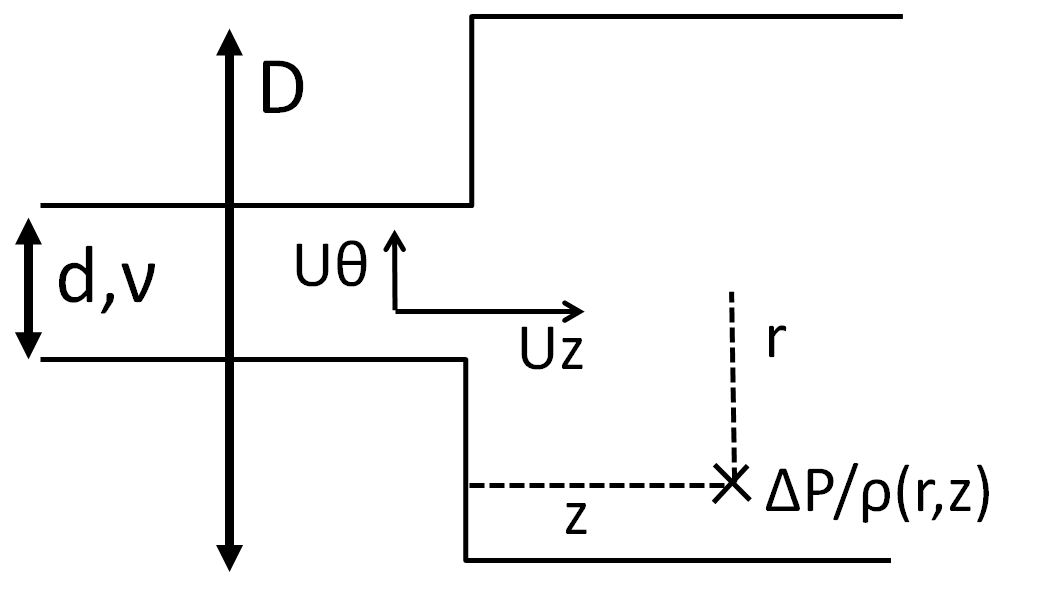
\includegraphics[width=0.6\textwidth]{fig/Schema_Vashy2.png}
  \caption{With cylindrical coordinates}
 \label{Vaschy2}
\end{figure}
In the previous case, the parameter $\frac{\Delta P}{\rho}$ has been considered as a macroscopic one, since not depending on $z$ and $r$ (let us assume the symmetry of rotation by neglecting $\theta$) . Let us now consider the case where we want to study a field depending on cylindrical coordinates : now $\frac{\Delta P}{\rho}(r,z)$. 

If we use the same approach, we easily see that there are 2 more unknown, with the same amounts of units, we have just added two adimensional coordinates to the problem, for instance $r/D$ and $z/D$. The input physical parameters driving the phenomena are the same. Hence, this is not absurd not to consider some coordinates, but we still have to know that the field will depend on adimensional coordinates.

Here, we have : $\frac{\Delta P}{\rho}(r,z)=f(\frac{r}{D},\frac{z}{D},Re,S,\frac{d}{D})$

From now on, let us not consider the dependency of the cylindrical coordinates.

\section{With a quarl angle}

Since Paul Jourdaine \cite{paul_jourdaine_nom_effect_2016} has now shown the huge dependency on the flow of the quarl angle, we can add it in our dimensional analysis.

\begin{figure}[!h]
  \centering
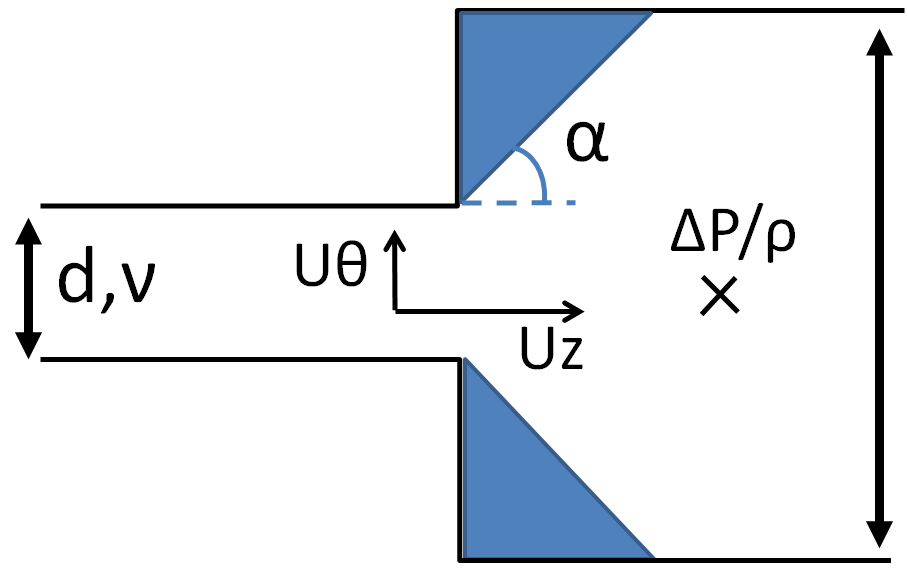
\includegraphics[width=0.6\textwidth]{fig/Schema_Vashy3.png}
  \caption{With quarl angle}
 \label{Vaschy3}
\end{figure}

The Vacshy-Buckingham analysis gives easily : that the quarl number is itself an adimen
sional number, we now have :
$\frac{\Delta P}{\rho}=f(\alpha,Re,S,\frac{d}{D})$


